\documentclass[aspectratio=169, 11pt]{beamer}

% ========== 主题设置 ==========
\usetheme{Madrid}
\usecolortheme{whale}
\setbeamertemplate{navigation symbols}{}
\setbeamertemplate{footline}[frame number]

% ========== 包 ==========
\usepackage{tikz}
\usetikzlibrary{arrows.meta, positioning, shapes.geometric, calc, fit, backgrounds}
\usepackage{booktabs}
\usepackage{graphicx}
\usepackage{amsmath}
\usepackage{xcolor}

% ========== 颜色定义 ==========
\definecolor{highlight}{RGB}{255, 100, 100}      % 当前工作模块(红色高亮)
\definecolor{completed}{RGB}{100, 200, 100}      % 已完成模块(绿色)
\definecolor{pending}{RGB}{200, 200, 200}        % 待完成模块(灰色)
\definecolor{inprogress}{RGB}{100, 150, 255}     % 进行中(蓝色)

% ========== 标题信息 ==========
\title{Weekly Progress Report}
\subtitle{Week 7: PhysioNet Joint Model \& Physical Arm Control}
\author{Student ID: 11314389}
\institute{BCI Control System Project}
\date{February 17, 2026}

\begin{document}

% ========== 标题页 ==========
\begin{frame}
    \titlepage
\end{frame}

% ========== Slide 1: 系统架构图 ==========
\begin{frame}{System Overview: Current Focus}
    \begin{center}
    \resizebox{0.95\textwidth}{!}{%
    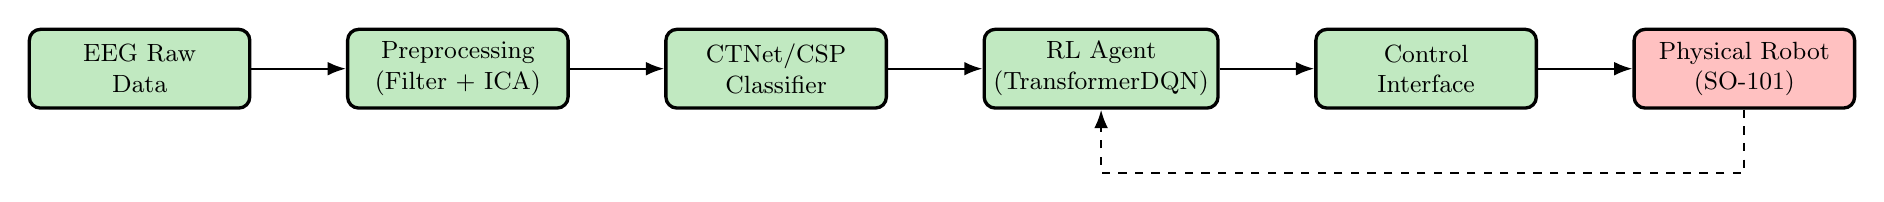
\begin{tikzpicture}[
        node distance=8mm and 12mm,
        block/.style={rectangle, rounded corners, draw, very thick,
                      minimum width=28mm, minimum height=10mm,
                      align=center, font=\small},
        arrow/.style={-Latex, thick},
    ]
        % 所有模块已完成!
        \node[block, fill=completed!40] (raw) {EEG Raw\\Data};
        \node[block, fill=completed!40, right=of raw] (prep) {Preprocessing\\(Filter + ICA)};
        \node[block, fill=completed!40, right=of prep] (csp) {CTNet/CSP\\Classifier};
        \node[block, fill=completed!40, right=of csp] (dqn) {RL Agent\\(TransformerDQN)};
        \node[block, fill=completed!40, right=of dqn] (ctrl) {Control\\Interface};
        \node[block, fill=highlight!40, right=of ctrl] (robot) {Physical Robot\\(SO-101)};
        
        \draw[arrow] (raw) -- (prep);
        \draw[arrow] (prep) -- (csp);
        \draw[arrow] (csp) -- (dqn);
        \draw[arrow] (dqn) -- (ctrl);
        \draw[arrow] (ctrl) -- (robot);
        
        % 反馈回路
        \draw[arrow, dashed] (robot.south) -- ++(0,-8mm) -| (dqn.south);
        
    \end{tikzpicture}}
    \end{center}
    
    \vspace{3mm}
    \begin{columns}[T]
        \column{0.5\textwidth}
        \textbf{Legend:}
        \begin{itemize}
            \item[\textcolor{completed}{\rule{8pt}{8pt}}] Completed
            \item[\textcolor{inprogress}{\rule{8pt}{8pt}}] In Progress
        \end{itemize}
        \column{0.5\textwidth}
        \begin{itemize}
            \item[\textcolor{highlight}{\rule{8pt}{8pt}}] \textbf{This Week's Focus}
            \item[\textcolor{pending}{\rule{8pt}{8pt}}] Pending
        \end{itemize}
    \end{columns}
\end{frame}

% ========== Slide 2: 本周目标 ==========
\begin{frame}{This Week's Objectives}
    \begin{block}{Goals Achieved}
        \begin{enumerate}
            \item \checkmark\ PhysioNet 联合模型训练 (20 被试, 73.89\% 准确率)
            \item \checkmark\ 添加早停机制防止过拟合
            \item \checkmark\ PhysioNet 数据集 RL 物理机械臂控制
            \item \checkmark\ Position vs Time 可视化添加到物理控制
        \end{enumerate}
    \end{block}
    
    \vspace{5mm}
    
    \begin{alertblock}{Key Achievement}
        PhysioNet 数据集现可用于 RL 物理机械臂控制,达到 \textbf{100\% 控制到达率}!
    \end{alertblock}
\end{frame}

% ========== Slide 3: PhysioNet 联合训练 ==========
\begin{frame}{PhysioNet Joint Model Training}
    \begin{columns}[T]
        \column{0.5\textwidth}
        \textbf{Training Configuration:}
        \begin{itemize}
            \item 被试数量: 20
            \item 样本总数: $\sim$900 trials
            \item 网络架构: SimpleCTNet
            \item 早停 patience: 30 epochs
            \item 最佳 epoch: 26
        \end{itemize}
        
        \vspace{3mm}
        \textbf{Early Stopping Mechanism:}
        \begin{equation*}
            \text{stop if } \text{Acc}_{\text{val}} \text{ no improve for } 30 \text{ epochs}
        \end{equation*}
        
        \column{0.5\textwidth}
        \textbf{Training Results:}
        \begin{table}
            \centering
            \small
            \begin{tabular}{lcc}
                \toprule
                Config & Subjects & Accuracy \\
                \midrule
                Single-subject & 1 & 77.78\% \\
                Joint (10 sub) & 10 & 67.78\% \\
                Joint (20 sub) & 20 & \textbf{73.89\%} \\
                \bottomrule
            \end{tabular}
        \end{table}
        
        \vspace{2mm}
        \textit{Early stopping prevented overfitting and saved best weights.}
    \end{columns}
\end{frame}

% ========== Slide 4: Physical Arm Control Results ==========
\begin{frame}{Physical Arm Control with PhysioNet}
    \begin{columns}[T]
        \column{0.55\textwidth}
        \textbf{Three-Dataset Comparison:}
        
        \vspace{2mm}
        \begin{table}
            \centering
            \small
            \begin{tabular}{lccc}
                \toprule
                Dataset & Ch & Class Acc & Control \\
                \midrule
                IV-2a & 22 & 63.19\% & 99.33\% \\
                IV-2b & 3 & 65.64\% & 98.00\% \\
                \textbf{PhysioNet} & 64 & \textbf{73.89\%} & \textbf{100\%} \\
                \bottomrule
            \end{tabular}
        \end{table}
        
        \vspace{3mm}
        \textbf{PhysioNet Physical Control:}
        \begin{itemize}
            \item Classification: 100\% (10/10)
            \item Control Reach: \textbf{100\%} (10/10)
            \item Avg Steps: 8.0
            \item Avg Reward: 10.32
        \end{itemize}
        
        \column{0.45\textwidth}
        \textbf{Key Observations:}
        \begin{itemize}
            \item 64-channel PhysioNet provides richest spatial info
            \item Joint model generalizes across 20 subjects
            \item RL compensates for classification errors
            \item Smooth velocity control prevents jitter
        \end{itemize}
        
        % Position vs Time 图可以在这里插入
        % \includegraphics[width=\textwidth]{../outputs/rl_physical_control/position_vs_time.png}
    \end{columns}
\end{frame}

% ========== Slide 5: 挑战与解决 ==========
\begin{frame}{Challenges \& Solutions}
    \begin{columns}[T]
        \column{0.5\textwidth}
        \begin{alertblock}{Challenges Encountered}
            \begin{itemize}
                \item 跨被试变异性导致过拟合
                \item 训练准确率 100\% vs 测试 67\%
                \item 机械臂运动抖动/限位碰撞
                \item 归位速度过慢
            \end{itemize}
        \end{alertblock}
        
        \column{0.5\textwidth}
        \begin{exampleblock}{Solutions Applied}
            \begin{itemize}
                \item 添加早停机制 (patience=30)
                \item 保存最佳权重而非最终权重
                \item SerialArmEnvV2: 速度控制 + 软限位
                \item 快速归位脚本 (velocity=500)
            \end{itemize}
        \end{exampleblock}
    \end{columns}
    
    \vspace{5mm}
    \begin{block}{Smooth Control Implementation}
        \texttt{move\_velocity=80} for slow smooth control, \texttt{velocity=500} for fast home/return
    \end{block}
\end{frame}

% ========== Slide 6: Code Structure Update ==========
\begin{frame}{Code Structure Update}
    \textbf{New/Modified Files:}
    
    \begin{columns}[T]
        \column{0.5\textwidth}
        \texttt{scripts/}
        \begin{itemize}
            \item \texttt{test\_physionet\_ctnet.py}
            \begin{itemize}
                \item Joint training mode
                \item Early stopping
                \item Model saving
            \end{itemize}
            \item \texttt{rl\_physical\_control.py}
            \begin{itemize}
                \item Position vs Time visualization
                \item PhysioNet support
                \item Joint model loading
            \end{itemize}
        \end{itemize}
        
        \column{0.5\textwidth}
        \texttt{Root/}
        \begin{itemize}
            \item \texttt{serial\_arm\_env\_v2.py}
            \begin{itemize}
                \item Velocity control
                \item Soft joint limits
                \item Auto-recenter
            \end{itemize}
            \item \texttt{outputs/physionet\_ctnet/}
            \begin{itemize}
                \item \texttt{physionet\_ctnet\_joint.pth}
            \end{itemize}
        \end{itemize}
    \end{columns}
\end{frame}

% ========== Slide 7: 下周计划 ==========
\begin{frame}{Next Week's Plan}
    \begin{block}{Planned Tasks}
        \begin{enumerate}
            \item 扩展动作空间:加入张开/闭合、移动等动作
            \item 下载更多被试 (50+) 进一步提升模型
            \item 跨被试泛化实验 (Leave-One-Subject-Out)
            \item 完善 Methodology 文档
        \end{enumerate}
    \end{block}
    
    \vspace{5mm}
    
    \begin{columns}[T]
        \column{0.5\textwidth}
        \textbf{Expected Deliverables:}
        \begin{itemize}
            \item 扩展动作的物理演示
            \item 更大数据集的训练结果
            \item Position vs Time 对比图
        \end{itemize}
        
        \column{0.5\textwidth}
        \textbf{Questions for Supervisor:}
        \begin{itemize}
            \item 是否需要 Leave-One-Subject-Out 验证?
            \item 对扩展动作空间的建议?
        \end{itemize}
    \end{columns}
\end{frame}

% ========== Slide 8: 时间线 ==========
\begin{frame}{Project Timeline}
    \begin{center}
    \resizebox{0.9\textwidth}{!}{%
    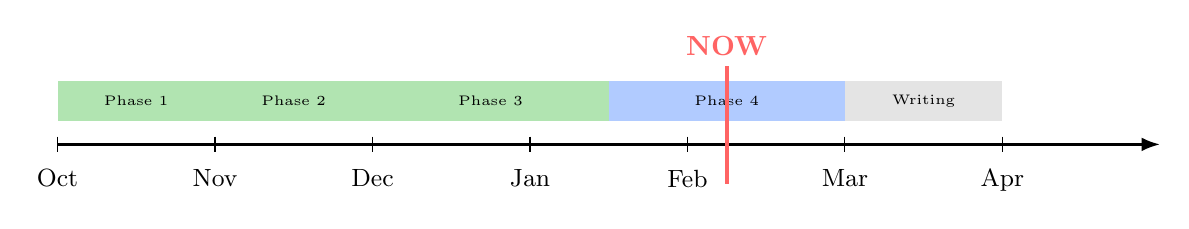
\begin{tikzpicture}
        % 时间轴
        \draw[thick, -Latex] (0,0) -- (14,0);
        
        % 月份标记
        \foreach \x/\month in {0/Oct, 2/Nov, 4/Dec, 6/Jan, 8/Feb, 10/Mar, 12/Apr} {
            \draw (\x, 0.1) -- (\x, -0.1);
            \node[below] at (\x, -0.2) {\small \month};
        }
        
        % 阶段块
        \fill[completed!50] (0, 0.3) rectangle (2, 0.8);
        \node at (1, 0.55) {\tiny Phase 1};
        
        \fill[completed!50] (2, 0.3) rectangle (4, 0.8);
        \node at (3, 0.55) {\tiny Phase 2};
        
        \fill[completed!50] (4, 0.3) rectangle (7, 0.8);
        \node at (5.5, 0.55) {\tiny Phase 3};
        
        \fill[inprogress!50] (7, 0.3) rectangle (10, 0.8);
        \node at (8.5, 0.55) {\tiny Phase 4};
        
        \fill[pending!50] (10, 0.3) rectangle (12, 0.8);
        \node at (11, 0.55) {\tiny Writing};
        
        % 当前位置
        \draw[highlight, ultra thick] (8.5, -0.5) -- (8.5, 1);
        \node[highlight, above] at (8.5, 1) {\textbf{NOW}};
        
    \end{tikzpicture}}
    \end{center}
    
    \vspace{3mm}
    \textbf{Current Status:} \textcolor{completed}{On track} -- Physical control validated on all 3 datasets!
\end{frame}

% ========== Summary Slide ==========
\begin{frame}{Summary}
    \begin{center}
    \Large
    \textbf{Key Achievements This Week}
    \end{center}
    
    \vspace{5mm}
    
    \begin{enumerate}
        \item \textbf{PhysioNet Joint Model}: 20 subjects, 73.89\% accuracy
        \item \textbf{Early Stopping}: Prevents overfitting, saves best weights
        \item \textbf{Physical Control}: 100\% success rate on PhysioNet
        \item \textbf{Position vs Time}: Visualization added for performance analysis
    \end{enumerate}
    
    \vspace{8mm}
    
    \begin{alertblock}{Milestone}
        \centering
        All 3 datasets (IV-2a, IV-2b, PhysioNet) successfully controlling physical SO-101 arm!
    \end{alertblock}
\end{frame}

\end{document}

